\documentclass[12]{article}

\usepackage{fullpage}
\usepackage{amsfonts}
\usepackage{amssymb}
\usepackage{amsmath}
\usepackage{graphicx}
\usepackage[margin=1in]{geometry}

\begin{document}

\begin{flushright}
8.6, 8.7, 8.8, 9.1 Write Up\\
Jim Vargas
\end{flushright}

\section{8.6 (8, 12)}
\textbf{(8): Find a power series representation for the function 
$\displaystyle{
f(x)=\frac{x}{2x^2+1}
}$ 
and determine the interval of convergence.
}
\begin{eqnarray}
f(x) &=& \frac{x}{2x^2+1}\\
&=& x\left(\frac{1}{1-(-2x^2)}\right)\\
\end{eqnarray}
Now, I will use the fact that
$\displaystyle{
\frac{1}{1-x} = \sum\limits_{n=0}^\infty x^n,\, \mathrm{for}\, |x|<1
}$
to write $f(x)$ as a sum $\Rightarrow$
\begin{eqnarray}
f(x) &=& x\sum\limits_{n=0}^\infty (-2x^2)^n\\
&=& \sum\limits_{n=0}^\infty (-1)^n\,2^n\,x^{2n+1}
\end{eqnarray}
I will use the Ratio Test to determine the interval of convergence. Let $a_n = (-1)^n\,2^n\,x^{2n+1}$:\\
\begin{eqnarray}
\lim\limits_{n\to\infty} \left|\frac{a_{n+1}}{a_n}\right| &=& \lim\limits_{n\to\infty} \left|\frac{(-1)^{n+1}2^{n+1}x^{2n+3}}{(-1)^n\,2^n\,x^{2n+1}}\right|\\
&=& |-2x^2| < 1\\
&=& 2|x|^2 < 1\\
&=& |x| < \sqrt{\frac{1}{2}}
\end{eqnarray}\\
The radius of convergence is $\sqrt{\frac{1}{2}}$. Now I will test the endpoints:
\begin{eqnarray}
\mathrm{When}\, x=\sqrt{\frac{1}{2}}\mathrm{:}&&\sum\limits_{n=0}^\infty (-1)^n\, 2^n\, \left[\left(\frac{1}{2}\right)^{(1/2)}\right]^{2n+1}\\
&=& \sum\limits_{n=0}^\infty (-1)^n\, 2^n\, (2^{-1})^{n+(1/2)}\\
&=& \sum\limits_{n=0}^\infty (-1)^n\, 2^{-(1/2)}
\end{eqnarray}
This can be shown to diverge using the Test for Divergence. let $a_n = (-1)^n 2^{-(1/2)}$:\\
$\displaystyle{
\lim\limits_{n\to\infty} a_n = \lim\limits_{n\to\infty} (-1)^n 2^{-(1/2)} \neq 0\mathrm{,\, therefore\,\, divergent.}
}$
\begin{eqnarray}
\mathrm{When}\, x=-\sqrt{\frac{1}{2}}\mathrm{:}&&\sum\limits_{n=0}^\infty (-1)^n\, 2^n\, \left[(-1)\left(\frac{1}{2}\right)^{(1/2)}\right]^{2n+1}\\
&=& \sum\limits_{n=0}^\infty (-1)^n\, (-1)^{2n+1}\, 2^n\, (2^{-1})^{n+(1/2)}\\
&=& \sum\limits_{n=0}^\infty (-1)^{3n+1}\, 2^{-(1/2)}
\end{eqnarray}
This can be shown to diverge using the same method above, so both endpoints diverge.\\
$\displaystyle{
\therefore\, f(x) = \sum\limits_{n=0}^\infty (-1)^n\,2^n\,x^{2n+1}
}$ on 
$\displaystyle{
I = (-\sqrt{\frac{1}{2}},\sqrt{\frac{1}{2}})
}$.

\textbf{(12): (a) Use the equation
$\displaystyle{
\frac{1}{1-x} = 1 + x + x^2 + x^3 + \cdots = \sum\limits_{n=0}^\infty x^x,\, |x|<1
}$ to find a power series representation for 
$f(x)=\ln{(1-x)}$. What is the radius of convergence?
}\\
\begin{eqnarray}
f(x) &=& \ln{(1-x)}\\
&=& -\int \frac{1}{1-x} \, dx
\end{eqnarray}
By the given equation, 
\begin{eqnarray}
f(x) &=& \int (-1 - x - x^2 - \cdots)\, dx  \\
&=& C + -x -\frac{x^2}{2} - \frac{x^3}{3} - \cdots\\
&=& C + \sum\limits_{n=1}^\infty \frac{-(x)^n}{n}
\end{eqnarray}
To determine $C$, $x=0$ can be put into the equation $\ln{(1-0)}=C$, so $C=0$. To determine the radius of convergence, the Ratio test can be used. Let $\displaystyle{
a_n = \frac{-(x)^n}{n}
}$:
\begin{eqnarray}
\lim\limits_{n\to\infty} \left|\frac{a_{n+1}}{a_n}\right| &=& 
\lim\limits_{n\to\infty} \left| \frac{-(x)^{n+1}}{n+1}\cdot \frac{n}{-(x)^n}\right|\\
&=& \lim\limits_{n\to\infty} \left| x\frac{n}{n+1} \right|\\
&=& |x| < 1
\end{eqnarray}
$\displaystyle{
\therefore\, f(x) =  \sum\limits_{n=1}^\infty \frac{-(x)^n}{n}
}$, $R = 1$.\\

\textbf{(12): (b) Use part (a) to find a power series for $f(x)=x\,\ln{(1-x)}$.
}
\begin{eqnarray}
f(x) &=& x\,\ln{(1-x)}\\
&=& x\sum\limits_{n=1}^\infty \frac{-(x)^n}{n}\\
&=& \sum\limits_{n=1}^\infty \frac{-(x)^{n+1}}{n}
\end{eqnarray}

\textbf{(12): (c) By putting $x=\frac{1}{2}$ in the result from part (a), express $\ln{(2)}$ as an infinite series.
}
\begin{eqnarray}
f\left(\frac{1}{2}\right) &=& \sum\limits_{n=1}^\infty \frac{-(\frac{1}{2})^n}{n}\\
&=& \frac{-1}{2} - \frac{1}{8} - \frac{1}{24} - \cdots	
\end{eqnarray}


\section{8.7 (32)}
\textbf{(32): Use a Maclaurin series to obtain the Maclaurin series for the function
$\displaystyle{
f(x) = \frac{x^2}{\sqrt{2+x}}
}$}\\
\begin{eqnarray}
f(x) &=& \frac{x^2}{\sqrt{2+x}}\\
&=&x^2(2+x)^{-1/2}\\
&=& \frac{x^2}{\sqrt{2}}(1+\frac{x}{2})^{-1/2}
\end{eqnarray}
Using the Binomial Maclaurin Series $\displaystyle{
(1+x)^k = \sum\limits_{n=0}^\infty \binom{k}{n} \,x^n
}$, $f(x)$ can be written as:
\begin{eqnarray}
f(x) &=& \frac{x^2}{\sqrt{2}}\sum\limits_{n=0}^\infty \binom{-1/2}{n} \left(\frac{x}{2}\right)^n\\
&=& \frac{x^2}{\sqrt{2}}\left[1 + (-1/2)(x/2) +\cdots+ \frac{(-1/2)(-3/2)(-5/2)\cdots(-1/2 - n+1)}{n!}(x/2)^n\right]\\
&=& \frac{x^2}{\sqrt{2}}\left[1 - \frac{x}{2^2} + \frac{(-1)^2(3)x^2}{2^4\cdot 2!}-\cdots+\frac{(-1)^n(3)(5)\cdots(2n-1)x^n}{2^{2n}\cdot n!}\right]\\
%&=& \frac{x^2}{\sqrt{2}}\left[1 +\sum\limits_{n=1}^\infty \frac{(-1)^{n}[(3)(5)\cdots(2n-1)]x^{n}}{2^{2n}\cdot n!} \right]\\
&=& \frac{x^2}{\sqrt{2}} \sum\limits_{n=0}^\infty \frac{(-1)^{n}[(3)(5)\cdots(2n-1)]x^{n}}{2^{2n}\cdot n!}\\
&=& \frac{1}{\sqrt{2}}\sum\limits_{n=0}^\infty \frac{(-1)^{n} \left[\prod\limits_{k=0}^{n-1} 2k+1 \right]x^{n+2}}{2^{2n}\cdot n!}
\end{eqnarray}
It is important to note here that an empty product 
$\displaystyle{
\prod\limits_{k=t+1}^t b_k
}$, that is, an infinite product where the upper limit is less than the lower limit, is equal to 1.

\section{8.8 (18)}
\textbf{ (18): (a) Approximate $f(x)=x\,\ln{(x)}$ by a Taylor Polynomial with degree 3 around $a=1$.
}\\

A Taylor Polynomial of degree three centered around $a$ is written as
$$\displaystyle{
f(x)\approx T_3(x) = f(a) + f^{(1)}(a)\frac{(x-a)}{1!} + f^{(2)}(a)\frac{(x-a)^2}{2!} + f^{(3)}(a)\frac{(x-a)^3}{3!}\,,
}$$
So the first three derivatives of $f(x)$ are needed.\\\begin{center}
\begin{tabular}{c|c|c}
$n$ & $f^{(n)}(x)$ & $f^{(n)}(1)$ \\ \hline
$0$ & $f^{(0)}(x) = x\,\ln{(x)}$ & $0$ \\ 
$1$ & $f^{(1)}(x) = \frac{1}{x}\cdot x + \ln{(x)}$ & $1$\\
$2$ & $f^{(2)}(x) = x^{-1}$ & $1$\\
$3$ & $f^{(3)}(x) = -x^{-2}$ & $-1$\\
$4$ & $f^{(4)}(x) = 2x^{-3}$
\end{tabular}\\
\end{center}
$f^{(4)}(x)$ is shown as well; it will be used later. So, The third degree Taylor Polynomial for $f(x)$ is 
$$\displaystyle{
f(x)\approx T_3(x) = 0 + \frac{(x-1)}{1!} + \frac{(x-1)^2}{2!} - \frac{(x-1)^3}{3!}
}$$
\textbf{ (18): (b) Use Taylor's Inequality to estimate the accuracy of the approximation $f(x)\approx T_3(x)$ when $.5\leq x\leq 1.5$.
}\\

Taylor's Inequality states that if $|f^{(n+1)}(x)|\leq M$ for $|x-a|\leq d$, then the remainder $R_n(x)$ of the Taylor series satisfies the inequality 
$$\displaystyle{
|R_n(x)|\leq \frac{M}{(n+1)!} {|x-a|}^{n+1},\,\,\mathrm{for}\, |x-a|\leq d
}$$
For this problem, $n=3$, $a=1$. Since $.5 \leq x \leq 1.5$, it follows that $-.5 \leq x-1 \leq .5$, so $|x-1|\leq .5$. In order to maximize $M$, and therefore $f^{(4)}(x)$, a small, positive number $<$ 1 is needed, so $x=.5$ can be used to find $M$:
\begin{eqnarray}
M &\geq & f^{(4)}(.5)\\
&\geq & \frac{2}{.5^3}\\
&\geq & 16
\end{eqnarray} 
Finally,
\begin{eqnarray}
|R_3(x)| &\leq & \frac{16}{4!}\cdot {.5}^4\\
&\leq & \frac{1}{24}
\end{eqnarray}
$\therefore R_3(x)$ of $[f(x)-T_3(x)]$ will not exceed .041$\bar{6}$ for $.5 \leq x \leq 1.5$.\\

\textbf{(18): (c) Check the result in (b) by graphing $|R_3(x)|$.}\\

The graph of $\displaystyle{
|R_3(x)| = \left|[x\,\ln{(x)}] - \left[\frac{(x-1)}{1!} + \frac{(x-1)^2}{2!} - \frac{(x-1)^3}{3!}\right]
\right|}$:\\
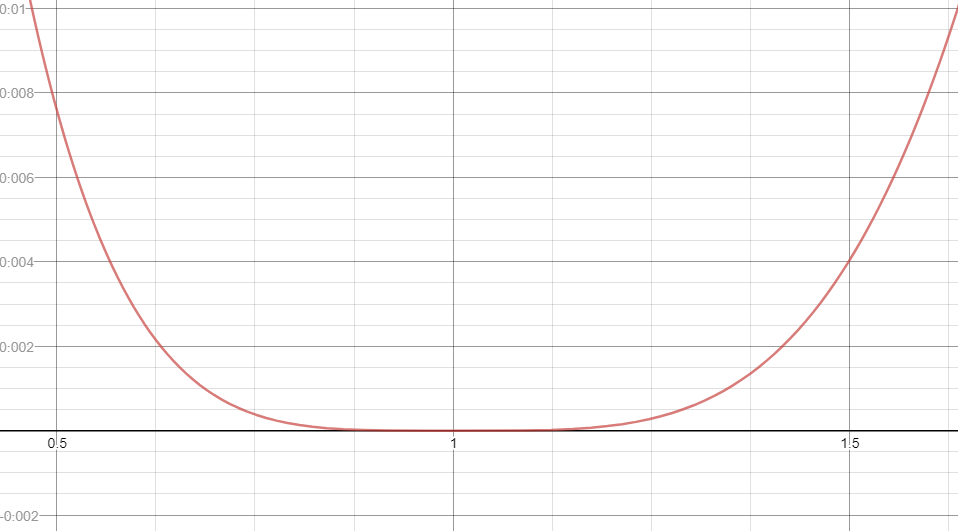
\includegraphics[scale=.5]{R_3(x).png}\\
From this graph, it seems that the error is less than about .008 for 
$.5 \leq x \leq 1.5$


\section{9.1 (16)}
\textbf{(16): Show that the equation 
$3x^2 + 3y^2 + 3z^2 = 10 + 6y + 12z$ represents a sphere, and find its center and radius.
}\\

The equation of a sphere is $(x-h)^2+(y-k)^2+(z-l)^2=r^2$, where $r$ is the radius and $(h,k,l)$ is the center of a circle. So,
\begin{eqnarray}
3x^2 + 3y^2 + 3z^2 &=& 10 +6y + 12z\\
3x^2 + 3y^2 - 6y + 3z^2 - 12z &=& 10\\
x^2 + (y^2 - 2y) + (z^2 -4z) &=& \frac{10}{3}
\end{eqnarray}
I will complete the squares:\begin{eqnarray}
y^2 - 2y &=& y^2 -2y +1 - 1\\
&=& (y-1)^2-1
\end{eqnarray}
\begin{center}and\end{center}
\begin{eqnarray}
z^2-4z &=& z^2-4z + 4 - 4\\
&=& (z-2)^2 -4
\end{eqnarray}
Now I substitute the values:
\begin{eqnarray}
x^2 + (y^2 - 2y) + (z^2 - 4z) &=& \frac{10}{3}\\
x^2 + ((y-1)^2 - 1) + ((z-2)^2 -4) &=& \frac{10}{3}\\
(x-0)^2 + (y-1)^2 + (z-2)^2 &=& \frac{10}{3} + 5\\
(x-0)^2 + (y-1)^2 + (z-2)^2 &=& \frac{25}{3}
\end{eqnarray}
This matches the equation for a sphere. The radius is $\displaystyle{\sqrt{\frac{25}{3}}}$ and the center is at $(0,1,2)$.

\end{document}